\documentclass{article}[12pt,a4paper]
\usepackage{graphicx}
\graphicspath{ {./images/} }

\title{Research Topic Proposal - Using Modern Micro-Controllers for Audio Modulation and Demodulation, Agnostic of Hardware}
\author{Joshua Jerred}
\date{\today}
\begin{document}
\maketitle

\section*{Introduction}

Historically, data modulation, for use in communication via radio, has been implemented in hardware. For each different type of modulation, you needed different hardware, both on the transmitting and receiving end. With the rise of more powerful computers, there has been a shift towards agnostic hardware that is given it's power through Software Defined Radio (SDR). Micro-controllers (MCUs), just like any other hardware, have continually become more computationally capable while also becoming cheaper and consuming less power. It seems that modern MCUs should be able to handle the task of audio modulation and demodulation in software, without the need for any modulation-mode specific hardware.

\section*{Background}

A paper published in 1998 by John Hansen, of State University of New York, talked about modulation of simple AX.25 packets on top of the AFSK modulation scheme, using PIC MCUs \cite{hansen_ax25}. John Hansen specifically mentioned using the PIC16F84 MCU. This is a 8-bit MCU with 1 KB of flash storage, 68 bytes of RAM, and runs at 20MHz\cite{pic_datasheet}. Since this time, ST has released the STM32 series of MCUs. These are 32-bit ARM Cortex-M MCUs which are just as affordable as the PIC MCUs were. A standard performance STM32, such as the STM32F4 series, has up to 2 MB of flash storage, 384 KB of RAM, and runs at up to 180 MHz\cite{st_datasheet}.

Audio Frequency Shift Keying (AFSK) is a method of modulating the frequency of a carrier signal to encode data. This modulation mode is commonly used in amateur radio applications, most commonly used alongside the AX.25 packet structure\cite{ax25_spec}. Traditionally modulating data at a rate of 1200 bits-per-second; it's not especially fast, but it can provide reliable data communication over long distances\cite{5167882}.

Often times a specialized bit of hardware, called a Terminal Node Controller (TNC), is used for AX.25 and AFSK implementation. These devices can range in price, normally starting out over \$150.

\section*{Rationale}

It seems as if the STM32 should be more than powerful enough to modulate and demodulate AFSK signals in software without support from any external hardware. This would show that common hardware that can be used to implement many different modes of data modulation.

Implementing AFSK modulation on a MCU has been done before\cite{8475994}, but non-embedded software was used for demodulation. This research would be to implement both modulation and demodulation on the same MCU allowing for a common hardware platform to be used on both ends of the communication link.

\section*{Hardware Considerations}
The only hardware requirement would be an STM32 that has at least one internal Digital-to-Analog converter (DAC) and at least one Analog-to-Digital converter (ADC). The easiest way to do this would be with an STM32 Nucleo board, a bit of hardware used for prototyping hardware design, similar to an Arduino. Availability is a concern, so a good choice would be the STM32F429ZI. ST sells a Nucleo prototyping board using this MCU. The F429 has the DACs and ADCs required for this task. Running at 180 MHz with 2 MB of flash, 256 KB of SRAM, it should be powerful enough to do so.

Using a Nucleo board will allow for a no hardware past a USB cable and 3.5mm audio jack. The F429 has a UART that can be accessed through the onboard ST-Link programming hardware, allowing a single USB connection to provide power and data communication with an external host. The external host/controller will be able to send and receive packets through a Virtual Comm Port on the UART interface.

\begin{center}
  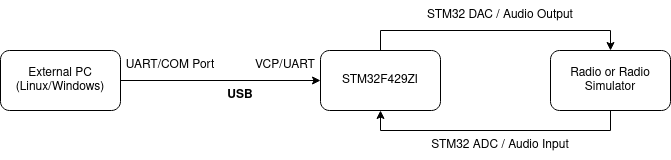
\includegraphics[width=4.5in]{images/hardware_outline.png}
\end{center}

\section*{Software Considerations}

Seeing as the time to complete this research is fairly short, the software stack should be kept simple. The following is the list of libraries that would be used in development.

\begin{itemize}
  \item[\textbf{STM32 HAL}]

  The STM32 Hardware Abstraction Library is a MCU specific library for interacting with the hardware inside the MCU. This would be used for core clock configuration, I/O pin configuration, ADC and DAC interfacing, and any other code that requires use of memory mapped hardware. Although it's not strictly required to use an STM32, it drastically reduces development time.

  
  \item[\textbf{STM32 USB/VCP}]
  The STM32 USB and Virtual Comm Port library is used for interfacing USB hardware with the MCU. In order to be able to communicate with the MCU externally, the STM32 USB/Virtual Comm Port library would be used so the host computer, running either Linux or Windows, would see the device as a generic serial device. This would be a simple method of communication that is still flexible. One thing to pay attention to using this method is the fact that there may be hardware interrupts driving the communication which could be a problem with real time audio generation and sampling.

  \item[\textbf{ETL}]
  ETL (Embedded Template Library) is a library that provides common functionality from the C++ standard library for embedded platforms. Although the standard library can be used, the ETL is mindful of memory management practices on embedded devices. The ETL avoids heap usage whenever possible as heap fragmentation is a concern when you are already working with so little RAM. One feature of the ETL is a hierarchical finite state machine structure (HFSM) that may be helpful in this use case.

  \item[\textbf{GCC Arm None ABI}]
  GCC Arm None ABI is a bare metal GCC compiler that supports ARM-Cortex platforms. Along with the compiler, there are basic templates that include bare minimum assembly entry point code for configuring the interrupt vector table and setting up an environment for C/C++ code prior to the call to main. Additionally there are template GCC linker files for each STM32 MCU that set up the address space and required sections in order to compile and run C/C++ code.

\end{itemize}

\bibliographystyle{plain}
\bibliography{refs.bib}

\end{document}